\section{Results}
\subsection{Quantitative results}

We will discuss our quantitative results in terms of the three measures that we have proposed earlier in the paper.

\subsubsection{Keystrokes Per Character (KSPC)}

\begin{figure}
    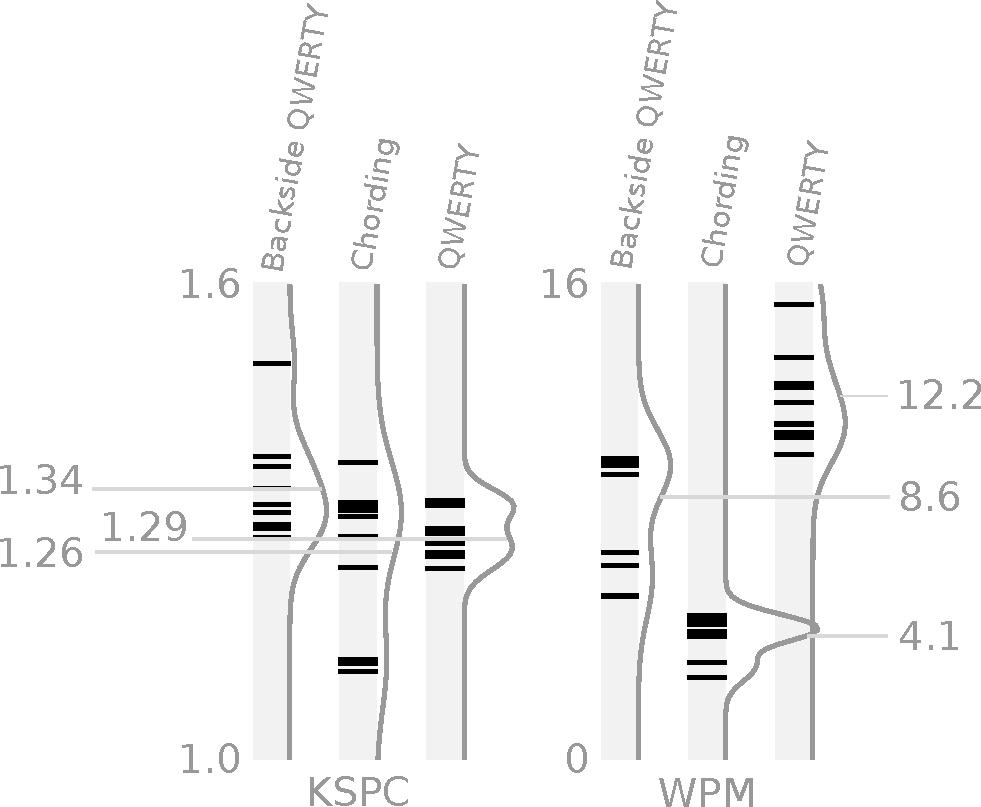
\includegraphics[width=0.5\textwidth]{Figures/kspc_and_wpm.pdf} 
    \caption{Keystrokes-per-character (KSPC) and words-per-minute (WPM) for each mechanism, with means noted. The continuous curves represent kernel densities of the population across ranges, 1.0-1.6 for KSPC and 0-16 for WPM. The tiny horizontal bars are scatter plots of individual measurements across the same ranges.}
    \label{fig:kspc_and_wpm}
\end{figure}
The Chording mechanism was on an average more accurate than the other two mechanisms, with the Backside QWERTY being the least accurate. An ANOVA pointed to a statistically significant main effect of the input technique on the KSPC ($F_{2,33}$ = 4.13, p$<$0.025). A two tailed t-test (for chording versus backside QWERTY) to validate this resulted in a p-value of 0.02, which essentially means that the chording mechanism was significantly more accurate than the backside-QWERTY. (Figure~\ref{fig:kspc_and_wpm}). 

\subsubsection{Words Per Minute (WPM)}

Our experiment findings suggested that QWERTY was still the fastest
mechanism, followed by backside QWERTY and the slowest was
chording. Statistics on WPM measurements can be found in
Figure~\ref{fig:kspc_and_wpm}. An ANOVA suggested a main effect of the input technique on the WPM. Pairwise comparisons suggested that QWERTY was faster than both backside QWERTY
and chording mechanisms. However, the test sessions were generally around 20-30 minutes, and each user only interacted with a mechanism once. Therefore, the fact that backside
QWERTY was on a average 3/4th as fast as the QWERTY mechanism was
encouraging. This led us to explore the results qualitatively and also
in terms of speed versus accuracy trade-off.


\subsubsection{Expert results}

Since the amount of exposure that the users received during the sessions was limited, it is obvious that lack of experience with the mechanisms also hampers the speed and accuracy measurements. Therefore, one of the researchers who was involved in development of the interface and had reasonable exposure to the interface went through the test in exactly the same fashion as the participants. This was done to test the capability of the two new mechanisms in terms of speed and accuracy. Table~\ref{tab:StatisticsForTestCorpora} shows the measurements from the same.  The results are also shown in Figure~\ref{fig:kspc_vs_wpm} for comparison.

\begin{table}
	\centering
		\begin{tabular}{rcc} 
		                         & \color{grey}{WPM}    & \color{grey}{KSPC} \\ 
                   \color{grey}{Chording} & 7.69   & 1.12 \\ 
                   \color{grey}{Backside QWERTY} & 13.231 & 1.152 \\ 
		\end{tabular}
	\caption{Sample Measurements}
	\label{tab:StatisticsForTestCorpora}
\end{table}

We can see from the table and figure that with decent amount of
exposure to the interface, both the accuracy and the speed seem to
improve, suggesting that there are strong learning trends which must
be considered. This concurs with claims made by previous text-input research on learning trends. \cite{LetterWise} 

\subsubsection{Speed versus Accuracy Trade-off}

\begin{figure}
    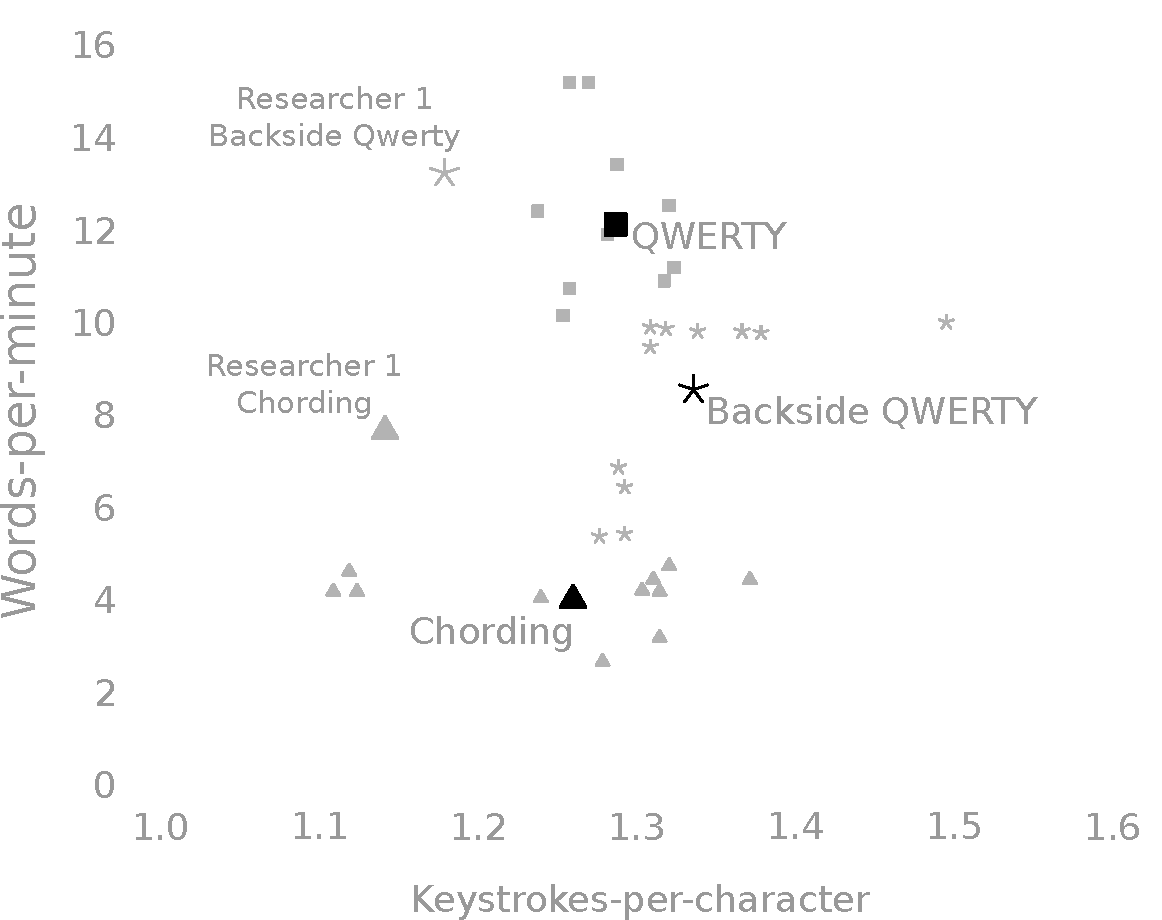
\includegraphics[width=0.5\textwidth]{Figures/kspc_vs_wpm.pdf} 
    \caption{Keystrokes-per-character (KSPC) vs. words-per-minute
      (WPM) for each mechanism.  The large symbols are the mean values
      for each individual mechanism. }
    \label{fig:kspc_vs_wpm}
\end{figure}

Examining the speed versus accuracy plot for each mechanism suggests that users reach a limit at which they cannot input data any faster, despite a sacrifice in accuracy (Figure~\ref{fig:kspc_vs_wpm}).  No user could break the 10wpm barrier with the Backside QWERTY mechanism, despite attempts over a wide range of accuracies.  We also had the same observation for the Chording mechanism.

Interestingly, there is a cluster of users who were able to achieve very high accuracy with the chording mechanism.  This was one of the primary design goals for the Chording mechanism: to reduce the dependency on precise physical positioning for accurate input.

We hypothesize that the ``speed-limit'' that users reach for the two novel mechanisms is partly due to the lack of kinesthetic memory (e.g. muscle memory) operating the keyboard, and unfamiliarity with the novel chording mechanism.  If this is the case, then concerted practice should result in faster performance.  Indeed, the results in Table~\ref{tab:StatisticsForTestCorpora} and Figure~\ref{fig:kspc_vs_wpm} show just that for at least one user. Since one user was able to break the ``speed-limit'' with extra practice, we suspect that the years of extra practice with the QWERTY mechanism is the primary source of the advantage that QWERTY enjoys.

The high accuracy rates of the Chording mechanism are therefore quite promising.  In the future, we will need to explicitly examine the impact of training time on speed and accuracy, and explore methods for accelerating users' acclimation to the unfamiliar input mechanism.

\subsubsection{NASA-TLX ratings}

As mentioned earlier, we used the NASA task load index to get subjective ratings on qualitative aspects of the interfaces. In the following few paragraphs we summarize the trends that were derived from the ratings that the participants assigned to the text-input mechanisms. Figure~\ref{fig:tlx-ratings} presents the ratings given by the users of all three mechanisms. It should be noted that the ratings range from 0-100 for each of the 6 dimensions (Mental demand, Physical demand, Temporal demand, Performance, Effort, Frustration). We ran one-way ANOVA tests on each of the 6 dimensions separately and combined (average of the 6). None of these tests resulted in a significant main effect of the input mechanism on the dimension under question (Table~\ref{tab:anova}). To summarize, a one-way ANOVA suggested that there was no significant main effect of the type of input technique on the perceived effective (average) workload ($F_{2,30}$ = 0.59, p$<$0.56). This result is encouraging and exciting as it implies that after the experiment, in spite of the slower speed, the users did not perceive the back-of-device input techniques as harder to perform. The result can also be qualitatively observed by the similarity in ratings exhibited in Figure~\ref{fig:tlx-ratings}.

\begin{table}
	\centering
		\begin{tabular}{rcc} 
		                         & \color{grey}{$F_{2,30}$}    & \color{grey}{p-value ($<$)} \\ 
                   \color{grey}{Mental Demand} & 1.74   & 0.19 \\ 
                   \color{grey}{Physical demand} &  0.65 & 0.52 \\ 
                   \color{grey}{Temporal demand} & 0.8 & 0.35 \\ 
                   \color{grey}{Performance} & 0.4 & 0.67 \\ 
                   \color{grey}{Effort} & 0.87 & 0.43 \\ 
                   \color{grey}{Frustration} & 0.36 & 0.7 \\ 
		\end{tabular}
	\caption{Table of ANOVA results}
	\label{tab:anova}
\end{table}


We also analyzed the recorded videos to explain some of the exceptions found in the NASA-TLX ratings. We observed that there were two users who gave the chording mechanism a rating implying that it did not have good performance. Both these participants had writing speeds that were less than the average. This suggests that these participants were struggling to get accustomed to the device and the mechanism, which might be a possible explanation for the low rating. We also looked at the videos from those sessions, and they corroborated the same claim. Moreover, the opinion on the amount of effort involved in working with the backside-QWERTY was less evenly distributed. However, for the chording it was almost evenly distributed around the average rating. The videos suggested that some of such cases were because the backside-QWERTY did not allow for change in size of the keyboard, people who had fingers longer or shorter than average finger sizes had a harder time with the mechanism as opposed to other. The chording mechanism on the other hand, did allow for such changes and therefore possibly got an even distribution of ratings.

\subsection{Qualitative results}
As mentioned earlier, we conducted post-session interviews to get some qualitative feedback. Apart from feedback on the mechanisms, in these interviews we tried to find users' opinion on the problems of occlusion and posture mentioned earlier.
\subsubsection{Backside QWERTY}
In the post-session interviews 8 out of 12 participants said that they felt that they were more comfortable in holding the device, in contrast to their experiences with a tablet form-factor device.
Only 3 out of 12 participants said that they felt their grip stability was being minimized when they reached out for a character. Moreover, 2 out of these 3 participants suggested having physical "strap-on" holders for fingers on the side to solve this problem. All the participants said that the mechanism solved the problem of occlusion, as all of the activity was happening at the back of the device. Moreover, 10 out of these 12 participants said this was a welcome change, the rest said they were indifferent.
\subsubsection{Chording mechanism}
In the post-session interviews 11 out of 12 participants said that they felt they were more comfortable in holding the device. None of the participants said that their grip stability was effected. In fact all the participants said that they felt that the mechanism was slow, but involved less movement and greater accuracy. As in the case of backside QWERTY all the participants said that the mechanism solved the problem of occlusion. Moreover, 8 out of 12 participants said the mechanism could be a welcome change, 3 of them said it might be too much work, and 1 of them was indifferent.

In spite of being self-reported, these qualitative observations strongly point towards the possibility that the two new mechanisms were able to solve the two major problems with text-input on devices with tablet form factor. Moreover, the fact that there was no perceived workload difference reported on the NASA-TLX and the results from WPM, KSPC measurements, these qualitative results look even more promising.

\begin{figure*}
    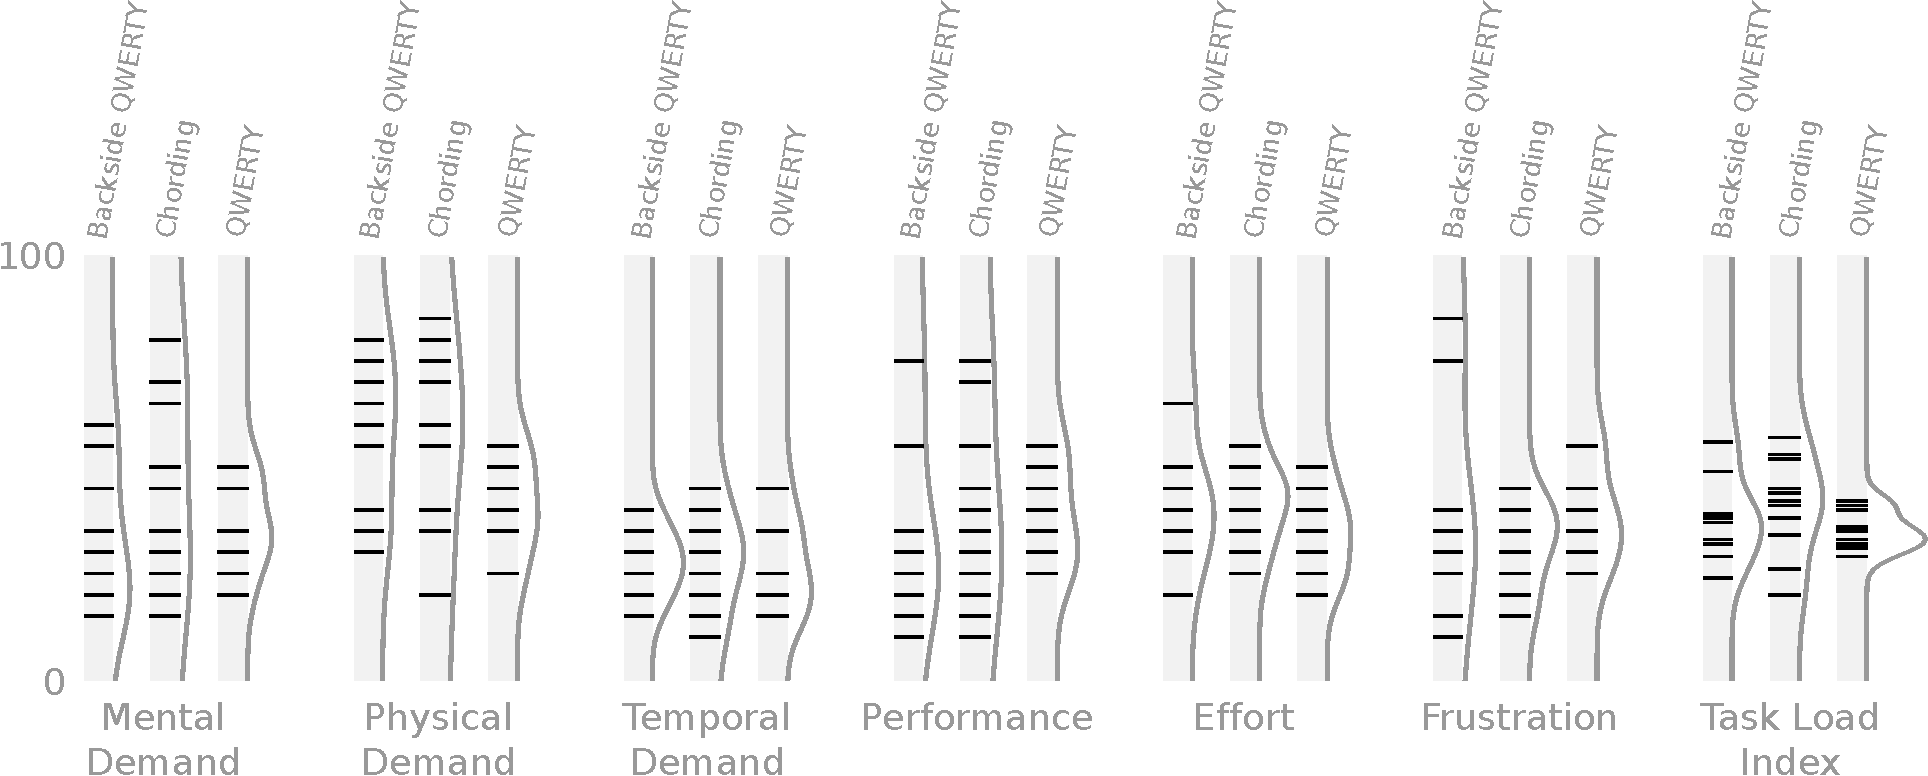
\includegraphics[width=\textwidth]{Figures/hash_and_densities_index.pdf} 
    \caption{NASA-TLX rating for all three input mechanisms}
    \label{fig:tlx-ratings}
\end{figure*}

\subsection{Design guidelines}

After a qualitative and quantitative analysis of our results, we also did a high-level analysis of our design choices and cross-checked them against the videos. As a result of this, we came up with some major design takeaways from this piece of research. Therefore, in this section we propose some design guidelines for future efforts that look into text input by utilizing a backside touch input device. 

\subsubsection{Movement minimization}

During the study we realized that the amount of movement involved in selecting a particular character determines the speed that users would achieve with the mechanism. The post-experiment analysis of usability test videos corroborated this claim. Once we reduced the size of the keys and magnified the movement of fingers, the users could cover larger distances with smaller shifts in position. We also realized that users are able to control the finger position with very high accuracy because their finger positions were anchored to the side of the device, and therefore these optimizations help them enter text at higher speeds.

\subsubsection{Multiple finger sizes}

There can be a lot of variation in finger sizes, amongst users. We accounted for this in the chording mechanism, by having settings that the user could select, if they had fingers larger or shorter than the average. This was critical for chording mechanism as the users were trying to form chords at specific locations. For backside-QWERTY, we did not make this optimization because users were not trying to position multiple fingers at the same time, and also because in that case we had tried to optimize between finger movement and key sizes.

\subsubsection{Reducing dimensions of movement}

This one is only true for the chording mechanism, but it turned out from the experiment that a good way to maximize on accuracy is to reduce the number of dimensions of movement. Traditionally, with a soft-QWERTY users tend to position themselves in both, x and y coordinate. In the chording mechanism, the y direction was being controlled by the number of fingers, and therefore the movement was just restricted to the x direction.

\subsubsection{Visual search vs Recall}

After the usability testing we also realized that without the tactile feedback of a keyboard, users tend to do a visual search to find characters instead of recalling from their previous experiences with QWERTY mechanisms. As long as the positions of characters follow a pattern, either pre-existing (like QWERTY) or familiar (alphabetic), users will be able to accustom themselves in a few interactions.

\subsubsection{Touch Cursors}
Our initial tests suggested that even though users use just one cursor at a given point of time to select a character, they still like to see the position of the rest of their fingers. This is because having a sense of the configuration of all the fingers, helps the users in relative positioning. Moreover, both our mechanisms involved showing finger positions on the screen and we had to this in a way that we don't hide any information or don't cause a loss of perception. We achieved this by doing a number of things. We made the touch cursors translucent, so that we don't occlude any information. We also kept the size of the cursor smaller than the size of an individual key so that they are easier to position and don't end up selecting multiple keys at the same time. 